
\section{背景：为什么电流子空间与材料更新之间还有一个问题}
电磁逆散射（electromagnetic inverse scattering，EIS）先用已知照明照射物体，再根据接收的散射场估计材料。正问题（forward problem）是材料已知时预测场；逆问题（inverse problem）是场已知时寻找材料。内部总场（total field）与感应电流（induced current）互相作用：材料响应产生电流，电流产生内部场，内部场又产生电流。

三维矢量Maxwell离散偶极子近似（discrete-dipole approximation, DDA）把物体离散成极化单元，每个单元保留三个场分量及并矢Green耦合（dyadic Green coupling，即三个分量之间的张量耦合）。离散方程解得精确，说明这个网格上的线性系统求解准确；与球体散射的独立Mie级数参考接近，才是在指定球体条件下检验连续散射。两者回答不同的问题。

子空间优化方法（subspace-based optimization method, SOM）利用接收Green算子的奇异结构辨认容易观测的电流。双重子空间优化方法（Twofold SOM, TSOM）进一步引入内部传播子空间；FFT-TSOM利用快速Fourier变换（fast Fourier transform, FFT）组织计算。这些方法已经考虑电流与材料的一致性以及内部作用。本文补上一个具体接口：改动一个既有电流子空间（current subspace）后，当前材料更新（material update）究竟怎样改变？

\begin{figure}[htbp]\centering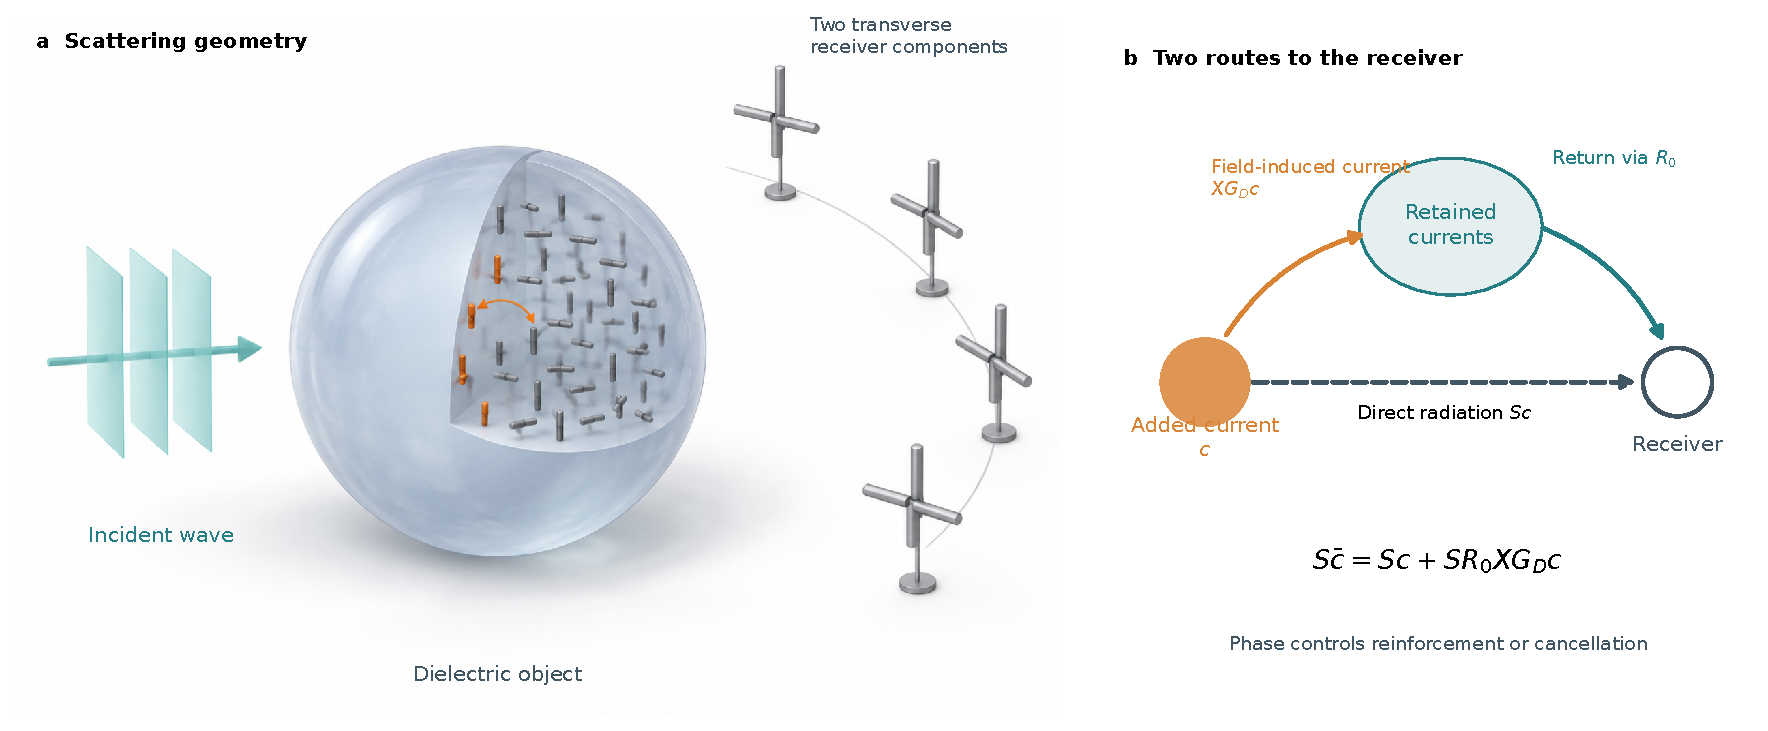
\includegraphics[width=.96\linewidth]{figures/physical_feedback.pdf}
\caption{材料、内部电流与接收的概念示意。新增电流有直接辐射和保留空间反馈两条返回路径；图中光线和局部电流是示意，不是计算场分布。}
\end{figure}

\section{从零读懂三条公式}
\subsection{材料扰动怎样到达接收器}
\[
J=SL^{-1}B.
\]
从右往左读：材料变化$s$通过真实注入（material injection）$Bs$形成电流激励；$L^{-1}$求全部多重散射（multiple scattering）后的电流变化；$S$计算接收响应。材料切向必须在体积加权的物理度量下正交化，复介电材料的实部和虚部是共享实变量。这样比较方向不会依赖人为参数单位。

\subsection{新增方向为什么不是只多一条直接辐射}
\[
\bar C=(I-R_0L)C=C+R_0XG_DC.
\]
这里$C$是新增电流方向，$R_0$是保留电流空间的求解算子，$X$是材料响应算子，$G_D$将电流变成内部场。右边第一项是新增方向本身，第二项是它激发保留电流后返回的响应。反馈（feedback）来自频域方程的消元。新增电流在内部产生场，保留电流对该场响应；二者的复振幅叠加后才到接收器。

\subsection{为什么完整材料步还要看残差}
\[
H_Us_U=-h_U,\qquad H_U=J_U^TJ_U+\Lambda,\quad h_U=J_U^Tr+\ell.
\]
曲率（curvature）描述材料方向的尺度和耦合；残差拉回（residual pullback）描述当前数据要求往哪个方向改；正则项（regularization）和线性prior项也参与。两个模型有相同$J^TJ$，仍可能有相反$J^Tr$。因此“模式信息强”还不足以决定它是否帮助当前材料步。

\section{如何读后面的实验}
完整GN差距是约化模型步相对同一完整模型最优步的二次误差。材料真值误差是估计材料与真实物体的物理距离。前者可以下降，后者仍可能上升，因为线性化、约束和步长尚需处理。

同一物体的三个状态、三个电流预算不是九个独立对象；同一计算五次计时也不是五份新物理证据。后面的表先按对象求和，再比较风险比；计时则单独衡量波动。读图时同时看绝对差距和相对比值，避免把越来越小的receiver分母误读为方法自身必然发散。
